\subsection{Regression}
The regression has been divided as a product of two sub models:
\begin{equation} \label{eq:regression_factor_equation}
B_{e hat} = B_{e factor} B_{e hat 0}
\end{equation}

Where $B_{ehat0}$ is zero speed regression and $B_{efactor}$ is a speed depending regression. Linear regression has been used for the two sub models. The feature selection, where the parameters of the regression has been selected has been carefully examined using cross validation. The data has been divided into a  training set (80\%) and a testing set (20\%). The selection has been made so that all tests with a specific ship model and its loading conditions are all in either the training set or the testing set. Only tests where there are results for both zero speed and at some speed for the same loading condition and ship model are included.    

100 random train/test sets were fitted and tested giving an average score: $mean(R^2)=0.66$, with standard deviation $std(R^2)=0.12$.

\begin{figure}[H]
    \centering
    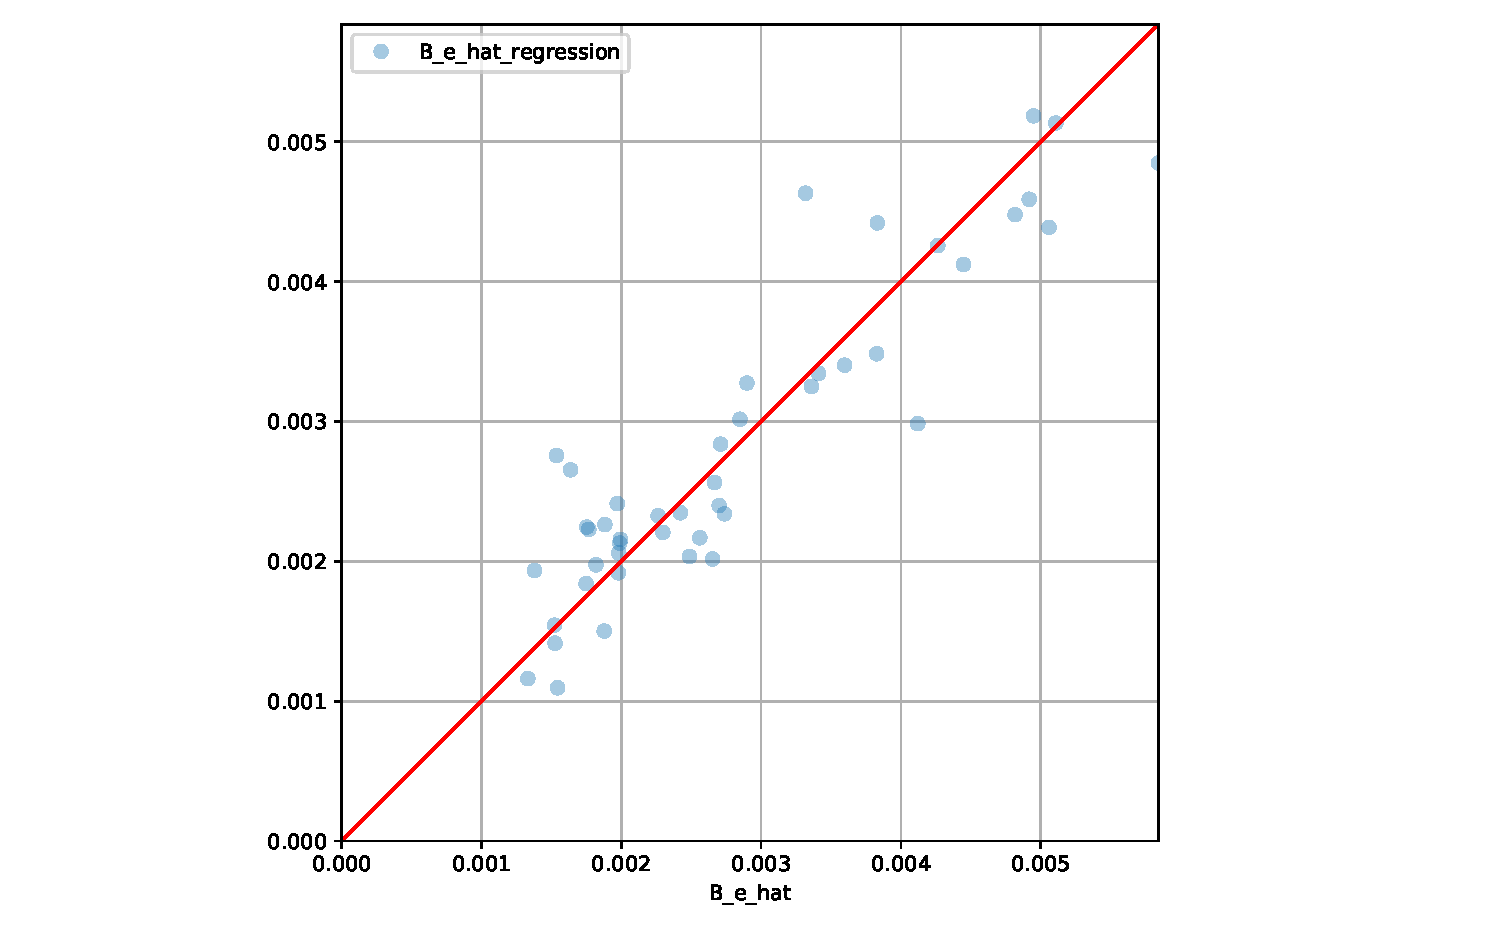
\includegraphics[width=\columnwidth]{figures/B_e_hat0_regression.pdf}
    \caption{Zero speed regression}
    \label{fig:B_e_hat0_regression}
\end{figure}

\begin{figure}[H]
    \centering
    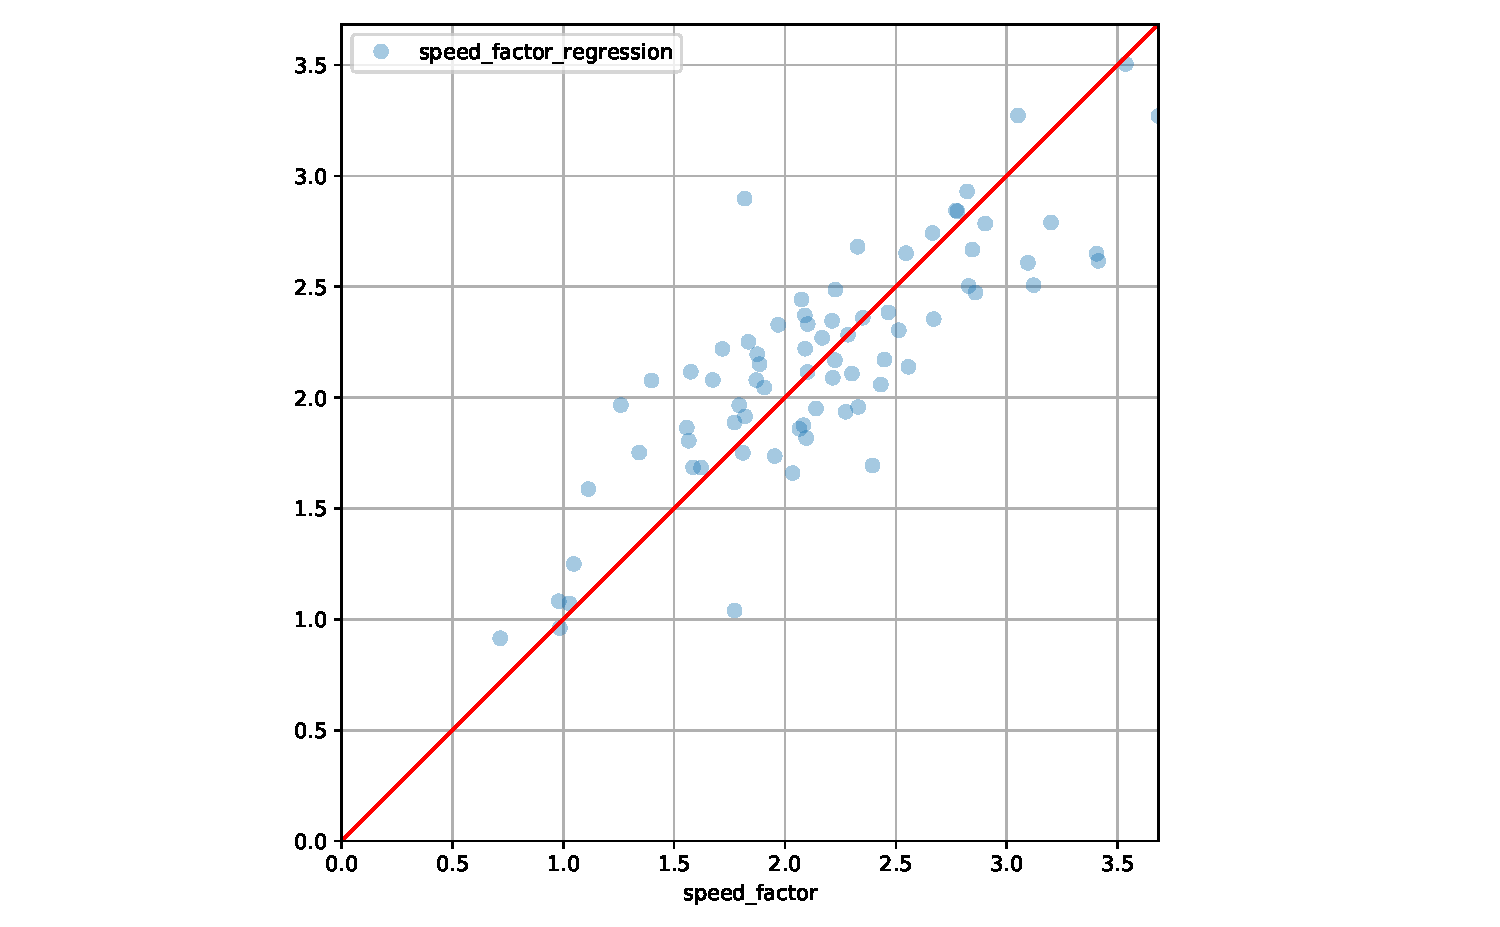
\includegraphics[width=\columnwidth]{figures/B_e_factor_regression.pdf}
    \caption{Speed dependency regression}
    \label{fig:B_e_factor_regression}
\end{figure}

\begin{figure}[H]
    \centering
    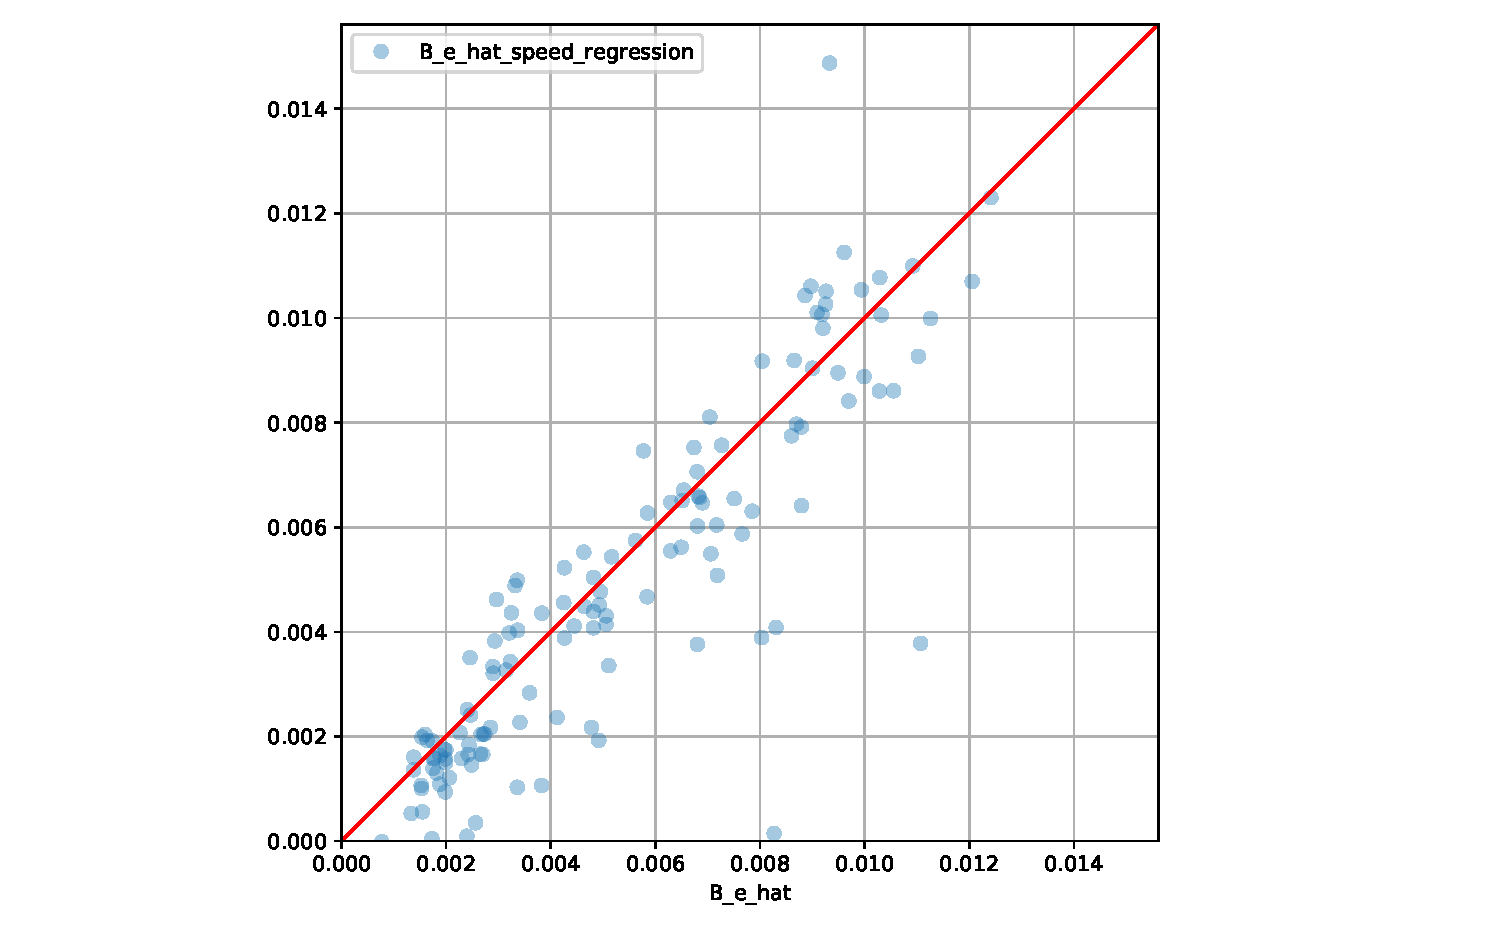
\includegraphics[width=\columnwidth]{figures/B_e_factor_regression_total.pdf}
    \caption{Total regression}
    \label{fig:B_e_factor_regression_total}
\end{figure}

\begin{equation} \label{eq:polynom_zero}
B_{e hat} = - 0.0136052800165908 A_{0} + 0.759326775676605 BK_{B} + 0.0725876320147426 GM - 0.0303297720484823 T + 0.00126493893040265 \omega_{0 hat} + 0.0143189616219315
\end{equation}

\begin{equation} \label{eq:polynom_speed}
B_{e factor} = 84.1 B_{L HAT} + 3.64 V + 0.468
\end{equation}
